% -*-coding: utf-8;-*-
% $Id: Part4.tex,v 1.9 2005-02-10 20:58:08 evlad Exp $
%%%%%%%%%%%%%%%%%%%%%%%%%%%%%%%%%%%%%%%%%%%%%%%%%%%%%%%%%%%%%%%%%
% Глава 4 - Прикладная часть + инструментальные программные средства
%%%%%%%%%%%%%%%%%%%%%%%%%%%%%%%%%%%%%%%%%%%%%%%%%%%%%%%%%%%%%%%%%

\label{mobile-robot}

\section{Описание робота}

Мобильный робот представляет собой тележку с тремя колесами, два из
которых расположены спереди и одно рояльное сзади.  Основные узлы
робота представлены на~\figref{fig:moby_projections}.  Передние колеса
являются ведущими и имеют независимые приводы $3$ и $4$.  Заднее
колесо расположено по средней оси платформы и не управляется.  Робот
оснащен системой технического зрения на основе видеокамеры $6$ с
инфракрасным фильтром.  Видеокамера закреплена неподвижно на
вертикальной мачте $7$.  На платформе также смонтированы компактный
компьютер $1$, система управления приводами $2$ и блок питания $5$.
Мобильный робот разработан сотрудниками и студентами кафедры
``Робототехнические системы и комплексы'' (РК-10)
МГТУ~им.~Н.~Э.~Баумана.

\begin{figure}[h]
\centerline{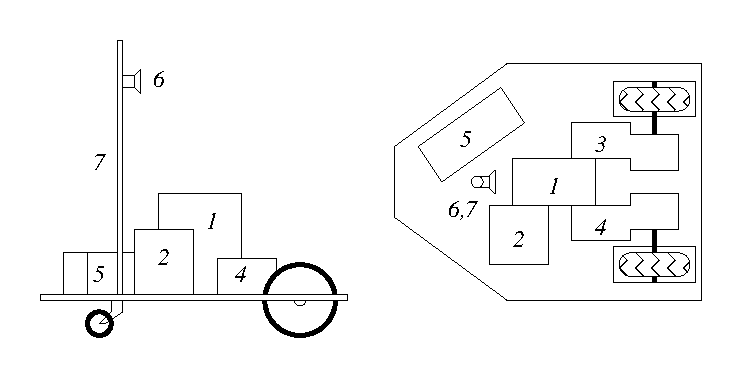
\includegraphics[width=0.8\textwidth]{moby_projections}}
\caption{Схема основных узлов мобильного робота (виды справа и сверху)}%
\label{fig:moby_projections}
\end{figure}

Каждый привод представляет собой двигатель постоянного тока, вал
которого связан с колесом через редуктор.  Известно, что
характеристики двигателей не идентичны.  В частности, одинаковое
напряжение, подаваемое на оба двигателя, приводит к разным скоростям
вращения валов.  Управление двигателями приводов осуществляется с
компьютера через блок $2$, преобразующим код широтно-импульсной
модуляции (ШИМ) в напряжение, подаваемое на двигатель.

Видеокамера является единственным сенсорным устройством мобильного
робота.  Изображение с камеры подается в компьютер робота через
специальный модуль, обеспечивающий оцифровку изображения.  Компьютер
мобильного робота PC-104 оснащен процессором Intel 486 и имеет
архитектуру типового ПК.  Компьютер может управляться как
непосредственно, при присоединении клавиатуры и монитора к блоку $1$,
так и удаленно через локальную сеть, поскольку робот оснащен сетевой
картой Ethernet.

Компьютер робота находится под управлением операционной системы QNX,
обеспечивающей параллельное выполнение задач в режиме реального
времени.  Операционная система поддерживает удаленное управление со
стационарного ПК по сети.  Для QNX имеются компиляторы языков высокого
уровня, в том числе {\sf C} и {\sf C++}, что позволяет удобно
реализовывать произвольные алгоритмы управления.

Управление роботом производится в дискретном времени, причем шаг
квантования времени определяется быстродействием управляющего
компьютера, выполняющего служебные процессы ОС QNX, а также прикладные
программы: процесс оцифровки изображения с видеокамеры с получением на
выходе координат маяка и процесс управления приводами на основе
полученных координат.  Протоколирование времени показывает, что один и
тот же фрагмент кода в циклической части программы управления
приводами исполняется на процессоре каждые 0.25 с.  Этот шаг
квантования соблюдается достаточно точно несмотря на параллельное
выполнение нескольких процессов, что свидетельствует о хорошем
качестве QNX как ОС реального времени.

\section{Задача движения на маяк}

Рассмотрим задачу управляемого движения робота на неподвижный маяк,
находящийся в поле зрения видеокамеры.  Обычно маяком выступает
висящая лампа накаливания, хорошо заметная в инфракрасных лучах.  Цель
робота --- за кратчайшее время оказаться как можно ближе к маяку.  Эта
задача является одной из типовых на ежегодном молодежном фестивале
``Мобильный робот''.

Будем считать, что в первый же момент времени один маяк находится в
поле зрения видеокамеры и по мере движения робота другие маяки в поле
зрения не попадают.  Таким образом, не будем рассматривать алгоритмы
поиска маяка и отождествления целевого маяка среди нескольких.

Рассмотрим решение задачи управляемого движения на маяк в
предположении, что координаты маяка в системе координат мобильного
робота неизвестны.  Робот ``видит'' маяк только посредством
видеокамеры, то есть, известно угловое отклонение робота от
направления на маяк.  Данной информации недостаточно для расчета
оптимальной траектории, по которой робот достигнет цели.  В этих
условиях единственно возможным является управление по отклонению от
направления на маяк.  Входом объекта управления в этом случае
выступает напряжение на приводах, а наблюдаемым выходом ---
горизонтальная координата маяка (с нулем в центре поля зрения
видеокамеры).

Первоначально управление мобильным роботом осуществлялось программным
П-регулятором с коэффициентом, подобранным оптимальным образом
эмпирическим путем.  Более сложные законы управления (ПИ, ПД, ПИД) не
были реализованы в силу трудности оптимизации их параметров.  Это
объективно объясняется существенной нелинейностью объекта управления,
проявляющейся даже на уровне кинематических
уравнений~\eqref{eq:alpha-far}.

Однако качество управления имеющимся регулятором оказалось
недостаточным при повышении требований к точности ``попадания''.
Задача повышения точности управляющего алгоритма особенно остро встала
в связи с управлением движением робота по сложному маршруту, когда
видимый маяк подменяется фиктивным, скользящим по целевой траектории
впереди мобильного робота.

Поскольку алгоритм управления по условию задачи не имеет информации о
приближении к маяку, цель управления --- минимизация ошибки
``попадания'' в маяк --- становится эквивалентной задаче минимизации
отклонения робота от направления на маяк по всей траектории движения.
Данная задача с учетом наличия удовлетворительно функционирующего
П-регулятора подходит для решения с помощью методики синтеза
квазиоптимального стохастического нейросетевого регулятора, описанной
в главе~\ref{neural_optimal_control}.

\subsection{Управление приводами}

Как уже отмечалось, робот оснащен двумя приводами ведущих колес,
независимо управляемыми с компьютера.  Для упрощения задачи будем
считать, что вместо двух каналов воздействия на объект (приводов)
имеется только один --- разница между напряжениями, подаваемыми на
приводы $\Delta u$  Назовем его {\it управляющим дифференциалом}.
$$\begin{array}{l}
u_L=u_0-\Delta u\\
u_R=u_0+\Delta u
\end{array}$$

Для обеспечения поступательного движения робота задается постоянное
значение напряжения $u_0$, подаваемого на приводы.  Для поворота
робота направо следует задать $\Delta u<0$.  В этом случае левое
колесо будет вращаться быстрее правого и робот будет поворачиваться
вправо.

\subsection{Локация маяка}

Поскольку робот перемещается в горизонтальной плоскости, нас будет
интересовать горизонтальная координата маяка в поле зрения
видеокамеры, принцип формирования которой в зависимости от положения
маяка иллюстрируется на \figref{fig:moby_eye_coord}.

\begin{figure}[h]
\centerline{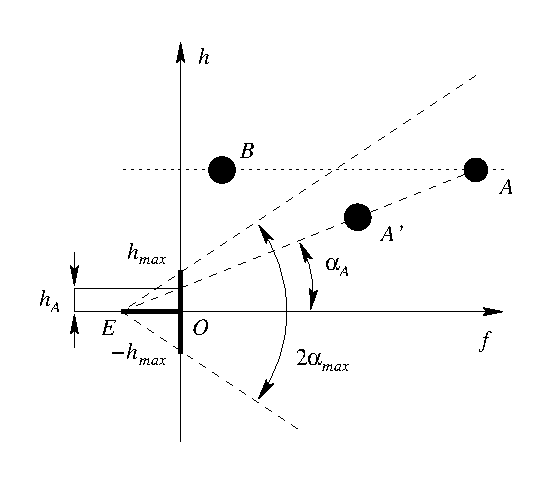
\includegraphics{moby_eye_coord_h}}
\caption{Координаты маяка в поле зрения видеокамеры мобильного робота
         (вид сверху)}
\label{fig:moby_eye_coord}
\end{figure}

Точка $E$ на схеме является воображаемым центром, в который сходятся
лучи из маяков.  Ось $f$ проходит через видеокамеру и совпадает с
направлением прямолинейного движения робота в текущий момент времени.
В силу ограниченности поля зрения видеокамеры углом $2\alpha_{max}$
маяки, расположенные в точках $A$ и $A'$, видны, а в точке $B$ нет.
На пути лучей имеется экран (поле зрения видеокамеры) с центром в
точке $O$.  Точка пересечения луча от маяка $A$ с экраном дает
координату $h_A$, поступающую из видеокамеры в компьютер.  Как угловая
координата $\alpha$ ограничена в диапазоне $[-\alpha_{max},
\alpha_{max}]$, так и отметка маяка на экране ограничена в диапазоне
$[-h_{max}, h_{max}]$.

Информация, поступающая в компьютер от видеокамеры, равномерно
дискретизирована от $-N\Delta h$ до $N\Delta h$, где $\Delta h$ ---
шаг дискретизации координаты маяка, а $2N$ --- число дискретных точек
на экране видеокамеры.  Очевидно, что равномерная дискретизация
экранных координат $h$ соответствует неравномерной дискретизации
угловой координаты $\alpha$.  Это одно из проявлений нелинейности
объекта управления.

По схеме видно, что угловые координаты маяков, расположенных в точках
$A$ и $A'$ совпадают при том, что расстояние до них разное.  Однако
видеокамера не в состоянии распознать различие.

Пример траектории движения мобильного робота на маяк в горизонтальной
плоскости $xy$ приводится на \figref{fig:moby_trajectory}а.

\begin{figure}[h]
\centerline{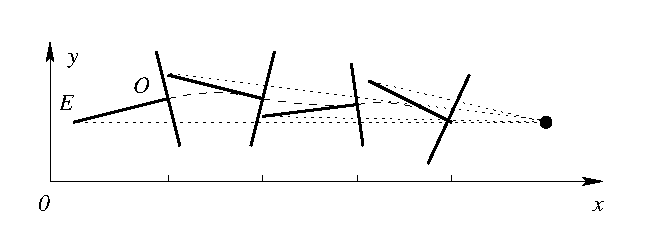
\includegraphics{moby_trajectory_a}}
\centerline{а)}
\centerline{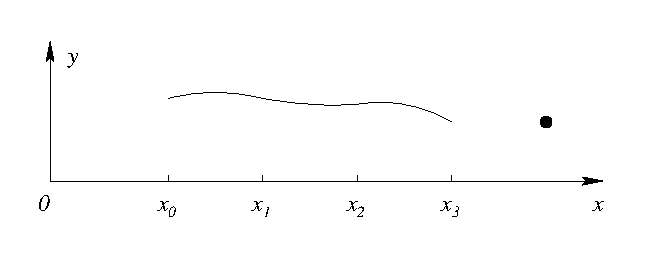
\includegraphics{moby_trajectory_b}}
\centerline{б)}
\centerline{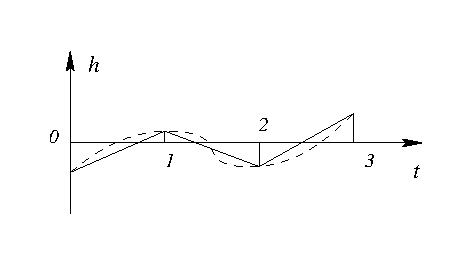
\includegraphics{moby_trajectory_c}}
\centerline{в)}
\caption{Траектория движения мобильного робота с промежуточными положениями
         платформы (а) и без них (б), а также траектория маяка в поле зрения
         видеокамеры (в)}
\label{fig:moby_trajectory}
\end{figure}


\section{Синтез нейросетевого регулятора}

Как уже отмечалось, оптимизация движения на маяк по угловому
отклонению без знания расстояния до маяка эквивалентна задаче
минимизации отклонения по траектории.  Учитывая это, можно применить
методику построения нейросетевого оптимального регулятора, изложенную
в предыдущих главах.  При этом объектом управления будем считать
систему с входом --- управляющим дифференциалом и наблюдаемым выходом
--- координатой маяка в поле зрения видеокамеры.

По методике для построения НОР необходимо решить следующие подзадачи:
\begin{enumerate}

\item наблюдать имеющуюся систему управления с целью сбора выборок,
      которые в дальнейшем будут использоваться для обучения нейронных
      сетей;

\item построить нейросетевую модель объекта управления при имеющемся
      регуляторе;

\item построить приближенный нейросетевой аналог действующего регулятора;

\item оптимизировать нейросетевой регулятор на основе инверсии объекта
      с помощью его нейросетевой модели.

\end{enumerate}



Для проверки функционирования нейросетевого регулятора при управлении
мобильным роботом и сравнения точности управления с исходным линейным
регулятором был проведен натурный эксперимент.  Сравнение точности
``попадания'' в маяк осуществлялось измерением минимального расстояния
от траектории робота до прекции маяка на горизонтальную плоскость.
Траекторией движения робота было решено считать след точки,
находящейся на передней кромке платформы по оси симметрии.  В этой
точке находился закрепленный карандаш, оставлявший след на листе
бумаги, расположенном под маяком.

\marginpar{Нужно ли и как измерять?}
Погрешность определения точки проекции маяка на лист бумаги составляет
5 мм (радиус груза отвеса).  Погрешность рисования траектории равна 1
мм (толщина грифеля карандаша).  Погрешность измерения минимального
расстояния от траектории до проекции маяка составляет 2 мм.

\subsection{Сбор обучающих данных}



\subsection{Нейросетевая модель мобильного робота}

\paragraph{Архитектура нейронной сети}
\paragraph{Обучение}

\subsection{Нейросетевое управление приводами}
\paragraph{Архитектура}
\paragraph{Предварительное обучение}
\paragraph{Окончательное обучение}

\subsection{Архитектура и обучение НС--Р}

\subsection{Сравнительный эксперимент}

\begin{table}
\caption{Величина промаха мимо маяка (в мм).}
\begin{tabular}{|l|r|l|}
\hline
Эксперимент & П-регулятор & НС-регулятор \\
\hline
1&	173&	58\\
2&	201&	47\\
3&	179&	22\\
4&	147&	57\\
5&	218&	29\\
6&	216&	72\\
7&	230&	39\\
8&	205&	40\\
9&	254&	44\\
0&	228&	79\\
11&	223&	79\\
12&	142&	40\\
13&	201&	77\\
14&	236&	53\\
15&	201&	29\\
16&	251&	29\\
\hline
Среднее&206.6&	49.6\\
СКО&	33.0&	19.1\\
\hline
\end{tabular}
\end{table}

\begin{itemize}

\item Архитектура НС--О: $\NN^o_{2+2,5,1}$

\item Архитектура НС--Р: $\NN^p_{1+1,5,3,1}$

\end{itemize}


В качестве траектории движения была   при его первом приближении к маяку.


\subsection{Обсуждение результатов}
\subsection{Выводы}

% Конец Главы 4
